\section{Motivating Examples}
\label{sec:examples}

In section~\ref{sec:method}, we presented a framework for constructing
an ROS (if deemed advantageous) by identifying unimportant parameters based on 
estimates of the screening metric, $\widehat{\mathcal{C}_i\mu_i}$
for individual parameters.
In this section, we motivate the underlying methodology by applying it to three
test problems,
namely, the borehole function, a non-linear oscillator, and a semilinear elliptic PDE.
Since model evaluations in all these test
problems are inexpensive, we compare relative importance of model parameters based
on the screening metric, obtained using model evaluations with 
converged estimates of $\mathcal{T}(\theta_i)$ based on the surrogate constructed in the
full parameter space (FSS). Additionally, to illustrate computational gains, we compare
convergence trends as a function of training runs for the ROS and the FSS using 
$\epsilon_{\mbox{\tiny LOO}}$ in Eq.~\ref{eq:loo}. 
Furthermore, as discussed earlier in section~\ref{sec:method}, we compare
PDFs of the model output, obtained using the ROS and the full-space surrogate for
the purpose of verification. 

\subsection{Borehole function}

The borehole function is a benchmark reference problem in sensitivity analysis.
It models the discharge of water ($\mathcal{Q}$) through a borehole in terms of
geometrical and physical parameters:
\be
\mathcal{Q} = \frac{\displaystyle
2\pi T_u(H_u - H_l)}{\displaystyle
\ln({r}/{r_w})\Big[1 +
\frac{2LT_u}{
\ln({r}/{r_w})r_w^2K_w} + \frac{T_u}{T_l}\Big]}
\label{eq:bore}
\ee
The radius of influence, $r$ is fixed at 3698.30 m whereas all other parameters
in the right hand side of~\eqref{eq:bore} are considered 
as uncertain. Hence, $\mathcal{Q} = \mathcal{Q}(\vec{\theta})$ with 
 $\vec{\theta} = (r_w, L, T_u, H_u, T_l, H_l, K_w)^T$, a vector of
 uncertain parameters. Table~\ref{tab:bore} provides distributions of the
 uncertain input parameters. 

\begin{table}[htbp]
\renewcommand*{\arraystretch}{1.2}
\begin{center}
\begin{tabular}{ll}
\toprule
\textbf{Parameter} & \textbf{Distribution} \\ 
\bottomrule
Borehole radius, $r_w$ (m) & $\mathcal{N}$(0.1,0.016) \\
Borehole length, $L$ (m) & $\mathcal{U}$[1120,1680] \\
Transmissivity of upper aquifer, $T_u$ (m$^2$/yr) & $\mathcal{U}$[63070,115600] \\
Potentiometric head of upper aquifer, $H_u$ (m) & $\mathcal{U}$[990,1110] \\
Transmissivity of lower aquifer, $T_l$ (m$^2$/yr) & $\mathcal{U}$[63.1,116] \\
Potentiometric head of lower aquifer, $H_l$ (m) & $\mathcal{U}$[700,820] \\
Borehole hydraulic conductivity, $K_w$ (m/yr) & $\mathcal{U}$[9855,12045] \\
\bottomrule
\end{tabular}
\end{center}

\caption{Description and distributions of uncertain parameters in the borehole function
given by~\eqref{eq:bore}.}
\label{tab:bore}
\end{table}
%
Cheap function evaluations of the discharge $\mathcal{Q}(\vec{\theta})$ using
enables computing accurate estimates of $\mathcal{T}(\theta_i)$ through
sampling, with a sufficiently large Monte Carlo sample size.  Shown in
Figure~\ref{fig:sense_bore}~(left) are estimates of these indices corresponding to the
uncertain parameters in the borehole function using 10$^6$ pseudo-random
samples in the input parameter space. 
%\footnote{Although $\mathcal{T}(\theta_i)$ might converge with much fewer
%samples depending upon the model, we consider a large number that typically
%ensures a converged estimate for the purpose of illustration.} 
These estimates are used to verify fidelity of
parameter screening based on the methodology presented in Section~\ref{sec:method}. 

\begin{figure}[htbp]
 \begin{center}
  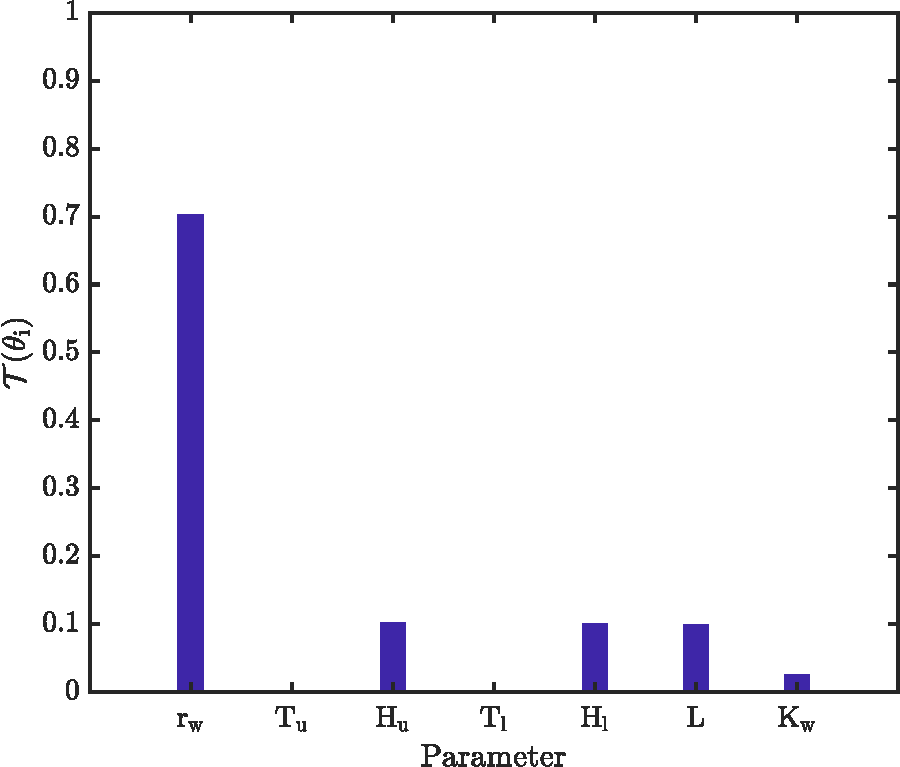
\includegraphics[width=0.48\textwidth]{./Figures/sense_borehole}
  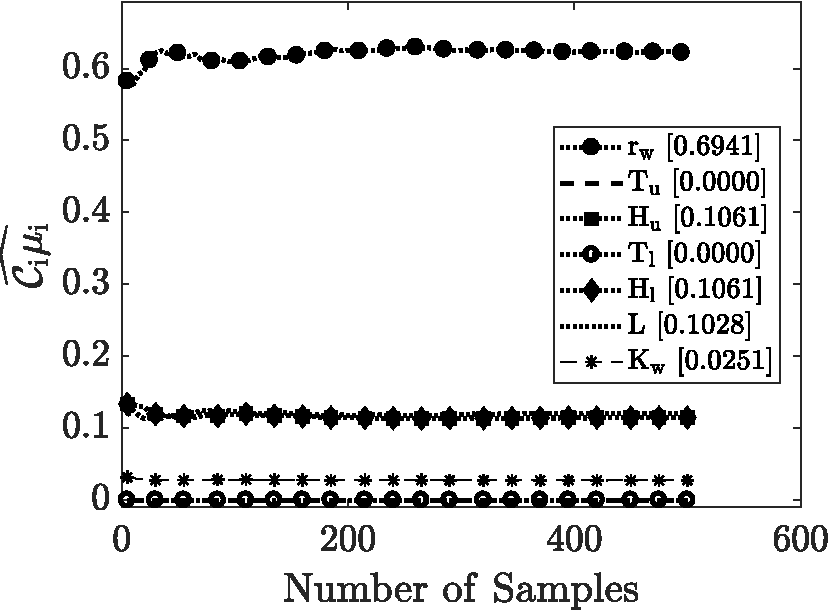
\includegraphics[width=0.51\textwidth]{./Figures/ub_conv_borehole}
\caption{
Left: Sobol' total sensitivity index, $\mathcal{T}(\theta_i)$ for uncertain
parameters in the
borehole discharge function in~\eqref{eq:bore}. Right: 
Estimates of the screening metric ($\widehat{\mathcal{C}_i\mu_i}$), plotted
against number of samples. Also included in the legend are estimates of
$\mathcal{T}(\theta_i)$ in each case in the legend.}
\label{fig:sense_bore}
\end{center}
\end{figure}

In Figure~\ref{fig:sense_bore}~(right), we plot estimates of the screening parameter 
$\widehat{\mathcal{C}_i\mu_i}$ for a wide range of the number of 
samples used for approximating $\mu_i$ using~\eqref{eq:mu}.
Estimates for $\widehat{\mathcal{C}_i\mu_i}$ are found to be in excellent agreement
with $\mathcal{T}(\theta_i)$ even when small number of samples (5--10) are used. 
Consequently, the relative importance of uncertain 
parameters in the borehole function is found to be consistent 
with predictions based on the Sobol' index. 
In the considered intervals for the uncertain parameters, it is clear 
that the discharge is insensitive to $T_u$ and $T_l$. 
Moreover, the sensitivity to $K_w$ is also small. We exploit these findings to reduce
the dimensionality of the problem by 
discounting the uncertainties in $T_u$, $T_l$, and $K_w$ by fixing 
them at their respective nominal values. 

Our goal as discussed is to gain computational advantage by constructing
surrogates in a reduced input parameter space. To this end, we use LAR to 
construct PCEs
in 5D and 4D spaces by fixing $\{T_u,T_l\}$ in the former and additionally
fixing $K_w$ in the latter at their respective mean values. In
Figure~\ref{fig:conv_bore}~(left), we compare convergence of PCEs constructed in the
full space (7D) with those constructed in the two reduced spaces (4D and 5D)
using $\epsilon_{\mbox{\tiny{LOO}}}$ (Eq.~\ref{eq:loo}). 

\begin{figure}[htbp]
 \begin{center}
  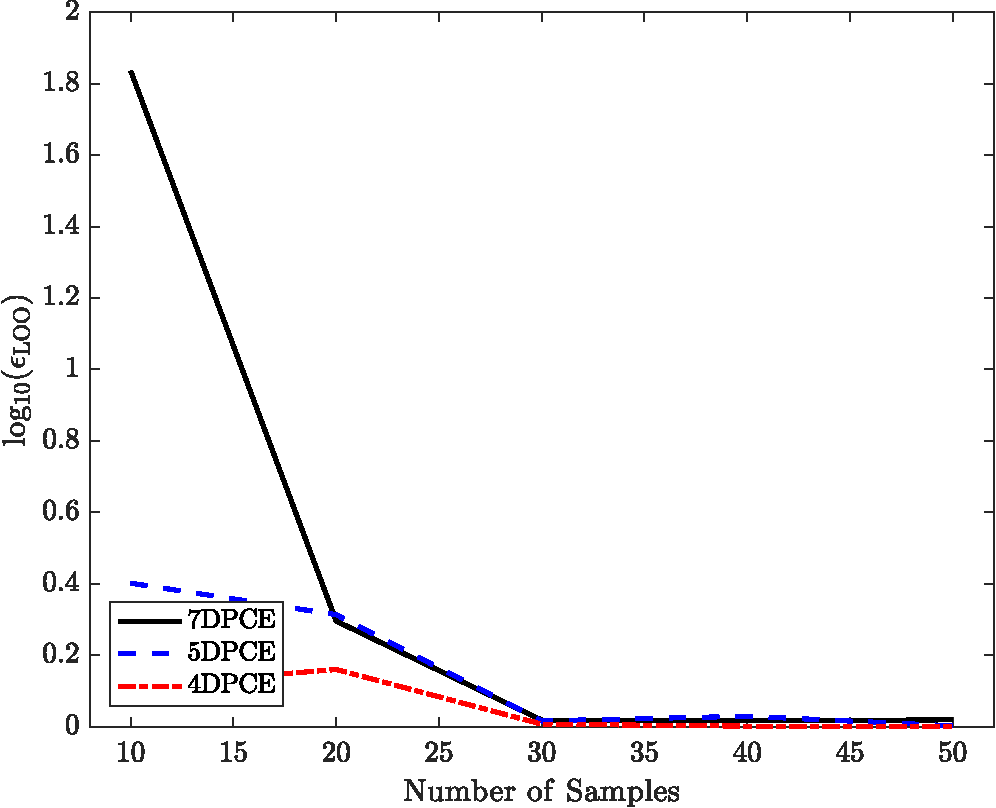
\includegraphics[width=0.48\textwidth]{./Figures/err_samples_borehole}
  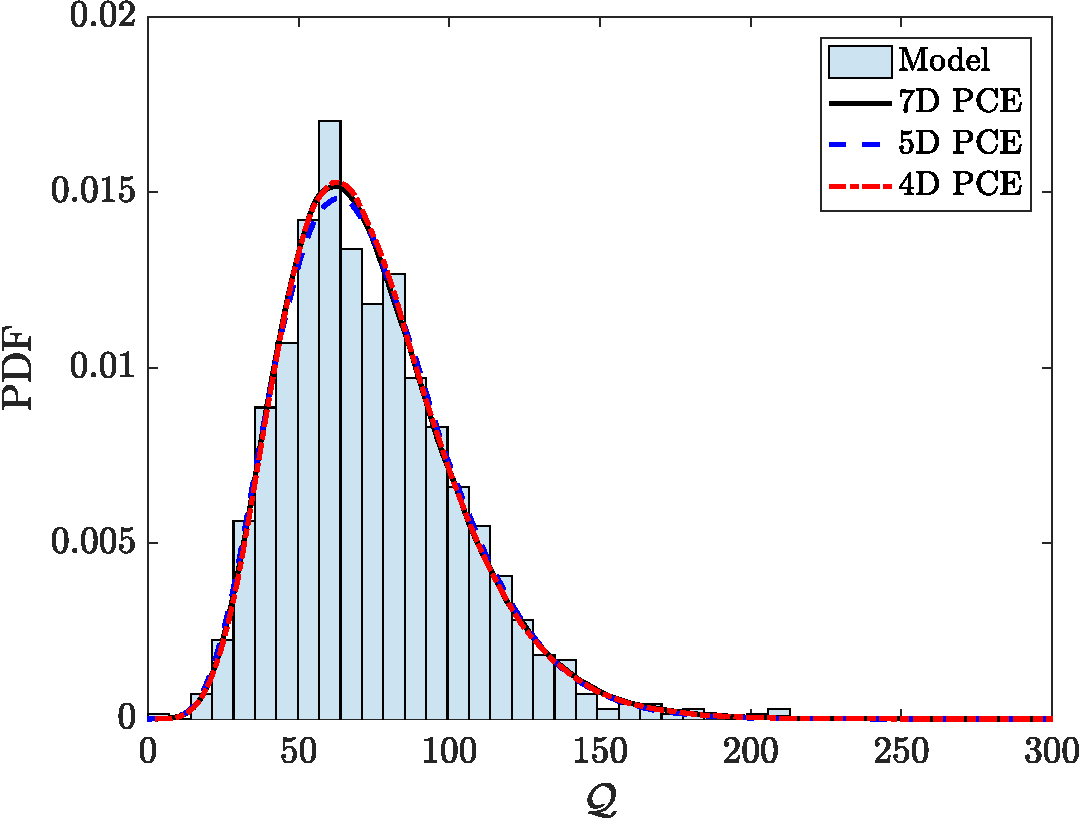
\includegraphics[width=0.48\textwidth]{./Figures/pdf_comp_borehole}
\caption{Left: A comparison of order of the leave-one-out-error 
($\epsilon_{\mbox{\tiny{LOO}}}$) as a function of number of regression samples
used for constructing the PCE in 4, 5, and 7 dimensions. Right: A comparison of
PDFs of the discharge, $\mathcal{Q}$, generated using 10$^{6}$ samples from
the marginal distributions of the uncertain parameters in each case.} 
\label{fig:conv_bore}
\end{center}
\end{figure}
%
As expected, it is observed that the PCE constructed in the 4D space converges
at a much faster rate. For instance, if a PCE with $\mathcal{O}(10^{-4})$
accuracy is sought, we need function evaluations at only about 50 sample points
in the 4D parameter space whereas the number of samples needed in the full 7D
space seems much higher. Latin hypercube sampling (LHS) was used in
each case. It must be pointed out that the error in Figure~\ref{fig:conv_bore}~(left)
is not expected to decrease monotonically with the increase in sample size
owing to the penalty term in the regularized optimization problem in Eq.~\ref{eq:reg}. 


As discussed earlier in this section, the reduced order PCE's are verified for
predictive accuracy in a least-squares sense and a probabilistic sense.
Estimates for $\epsilon_{\mbox{\tiny{L-2}}}$ based on 50 samples in the
validation test suite were
found to be 0.0551 and 0.0112 for the 4D and 5D PCE's respectively. In other
words, the 4D PCE is accurate within 5.52$\%$ and the 5D PCE is accurate within
1.12$\%$ of predictions based on the borehole function. We note  that although
the convergence in the case of a 5D PCE is slower (Figure~\ref{fig:conv_bore}),
its predictive accuracy is higher than the 4D PCE. This illustrates the
trade-off between accuracy and computational efficiency for the present 
problem. Generally, the required level of accuracy is problem dependent. 
The present framework allows for moving towards higher fidelity 
reduced order surrogates based on the ranking of the parameter sensitivities. 
 
%A possible explanation for this observation is that above a certain order
%of convergence, the uncertainty in $k_w$ contributes much more towards
%predictive accuracy of the reduced order PCE. It is therefore critical to
%account for the order of PCE convergence as well as its predictive accuracy for
%a given application, as highlighted earlier in section~\ref{sec:method}. 


Figure~\ref{fig:conv_bore}~(right) illustrates a comparison of the PDFs
of the
discharge, $\mathcal{Q}$ obtained by propagating 10$^6$ random
samples through the 7D PCE in the original input parameter domain as well as
the reduced order PCEs constructed in 4 and 5 dimensions. A normalized histogram
plot using 1000 model evaluations in the validation test suite is also included.
It is evident from this plot, that the PDFs agree quite favorably with each
other as well as the model-based histogram with respect to the modal estimate
as well as the uncertainty associated with $\mathcal{Q}$. 
Consequently, it can be said that the reduced order PCE is verified in a
probabilistic sense. In other words, the mode as well as the uncertainty in the
observable is reliably captured and predicted by the reduced order PCE. 
% 
\subsection{Nonlinear Oscillator}
We consider an undamped nonlinear oscillator with only one degree of
freedom as illustrated in Figure~\ref{fig:osc}. 
\begin{figure}[htbp]
 \begin{center}
  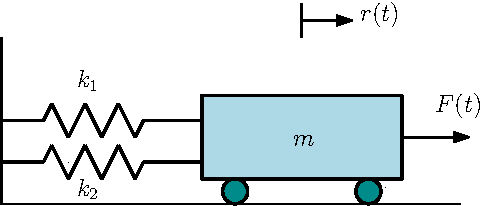
\includegraphics[width=0.5\textwidth]{./Figures/oscillator}
\caption{Schematic illustration of an undamped non-linear oscillator system with one degree of freedom.}
\label{fig:osc}
\end{center}
\end{figure}
This system has been studied extensively for its reliability using
the following state function~\cite{Bucher:1989,Bucher:1990,Rajashekhar:1993,Schueremans:2005,Gayton:2003}:
%
\be
g(\bm{X}) = 3r - \left|z_\text{max}\right| = 3r - 
\left|\frac{2F}{m\omega_0^2}\sin\left(\frac{\omega_0t_1}{2}\right)\right|,
\label{eq:limit}
\ee
\noindent where $z_\text{max}$ is the maximum displacement response of the system, $r$ denotes the displacement at
which either spring yields, $\bm{X}=(m,k_1,k_2,r,F,t_1)^T$ is the vector 
of uncertain parameters, and   
$\omega_0~=~\sqrt{(k_1+k_2)/m}$. The uncertain parameters are considered to be normally distributed with mean
and variance as provided below in Table~\ref{tab:osc}.

\begin{table}[htbp]
\renewcommand*{\arraystretch}{1.2}
\begin{center}
\begin{tabular}{ll}
\toprule
\textbf{Parameter} & \textbf{Distribution} \\ 
\bottomrule
Mass, $m$ (kg) & $\mathcal{N}$(1,0.05) \\
Time, $t_1$ (s) & $\mathcal{N}$(1,0.2) \\
Force, $F$ (N) & $\mathcal{N}$(1,0.2) \\
Displacement, $r$ (m) & $\mathcal{N}$(0.5,0.05) \\
Spring Constant, $k_1$ (Nm$^{-1}$) & $\mathcal{N}$(1,0.1) \\
Spring Constant, $k_2$ (Nm$^{-1}$) & $\mathcal{N}$(0.1,0.01) \\
\bottomrule
\end{tabular}
\end{center}

\caption{Description and distributions of uncertain parameters in the limit state function~\eqref{eq:limit}.}
\label{tab:osc}
\end{table}

Converged estimates of $\mathcal{T}(\theta_i)$ are once again obtained easily by
evaluating $g(\bm{X})$ for a large set of samples in the uncertain 
parameter space; see Figure~\ref{fig:sense_osc}~(left). Estimates of the screening metric, 
$\widehat{\mathcal{C}_i\mu_i}$ are plotted against the number of samples in 
Figure~\ref{fig:sense_osc}~(right). 
\begin{figure}[htbp]
 \begin{center}
  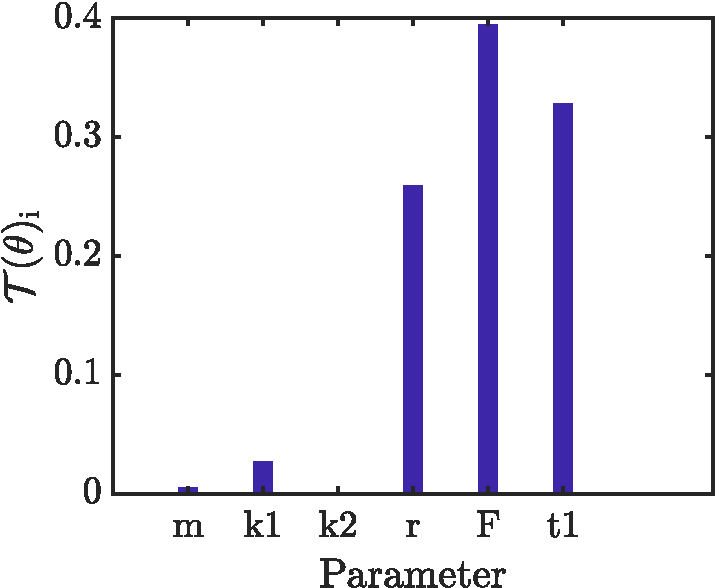
\includegraphics[width=0.48\textwidth]{./Figures/sense_oscillator}
  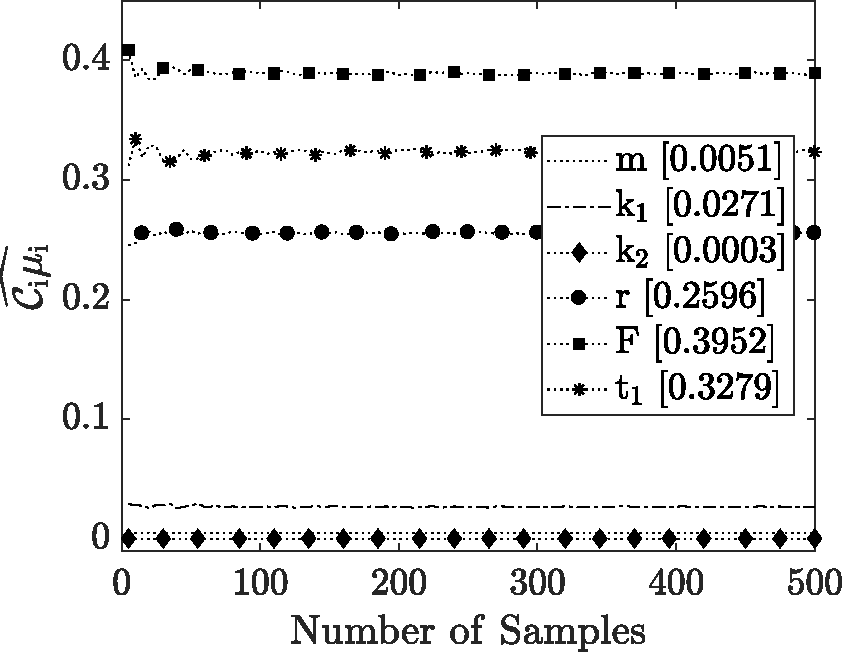
\includegraphics[width=0.48\textwidth]{./Figures/ub_conv_oscillator}
\caption{
Left: Sobol' total sensitivity index, $\mathcal{T}(\theta_i)$ for uncertain parameters in the limit 
state function in~\eqref{eq:limit}. Right: 
Estimates of the screening metric ($\widehat{\mathcal{C}_i\mu_i}$), plotted
against number of samples. Also included in the legend are estimates of $\mathcal{T}(\theta_i)$
in each case in the legend.}
\label{fig:sense_osc}
\end{center}
\end{figure}
We note that the total Sobol sensitivity indices are in excellent agreement
with the screening metric estimates. 
Consequently, the parameter ranks are found to be consistent in the
two plots in  
Figure~\ref{fig:sense_osc}.
It is observed that the limit state function is predominantly sensitive 
to $r$, $F$, and $t_1$. Hence, it seems likely that an ROS in
three dimensions is able to capture the overall uncertainty in $g(\bm{X})$.
% due to uncertainty in the six parameters. 
To illustrate computational gains as a
result of dimension-reduction, we construct PCEs in 3D, 4D (accounts for the
uncertainty in $k_1$ as well), and the original 6D parameter domain. In
Figure~\ref{fig:conv_osc}~(left), we compare the convergence of the
PCEs. As expected, the third-order PCE converges much faster than the other
two. Consequently, the number of model evaluations required for a converged PCE
is expected to be relatively much smaller in this case.  
\begin{figure}[htbp]
 \begin{center}
  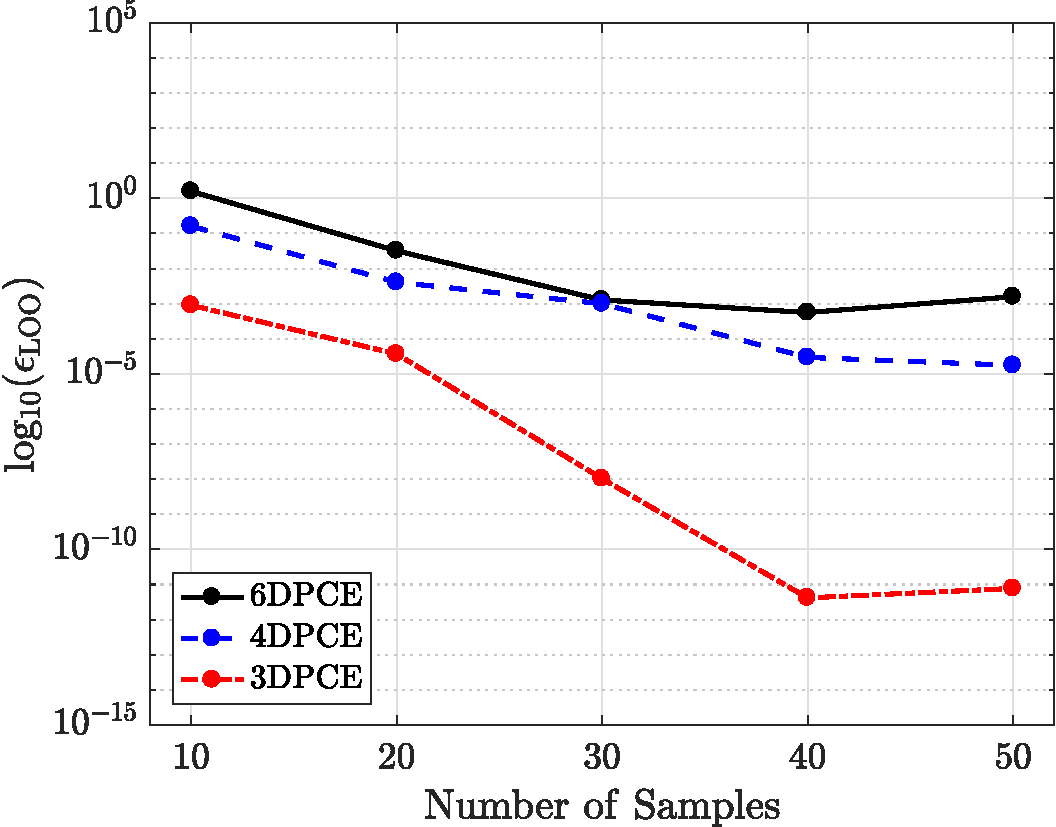
\includegraphics[width=0.48\textwidth]{./Figures/err_samples_oscillator}
  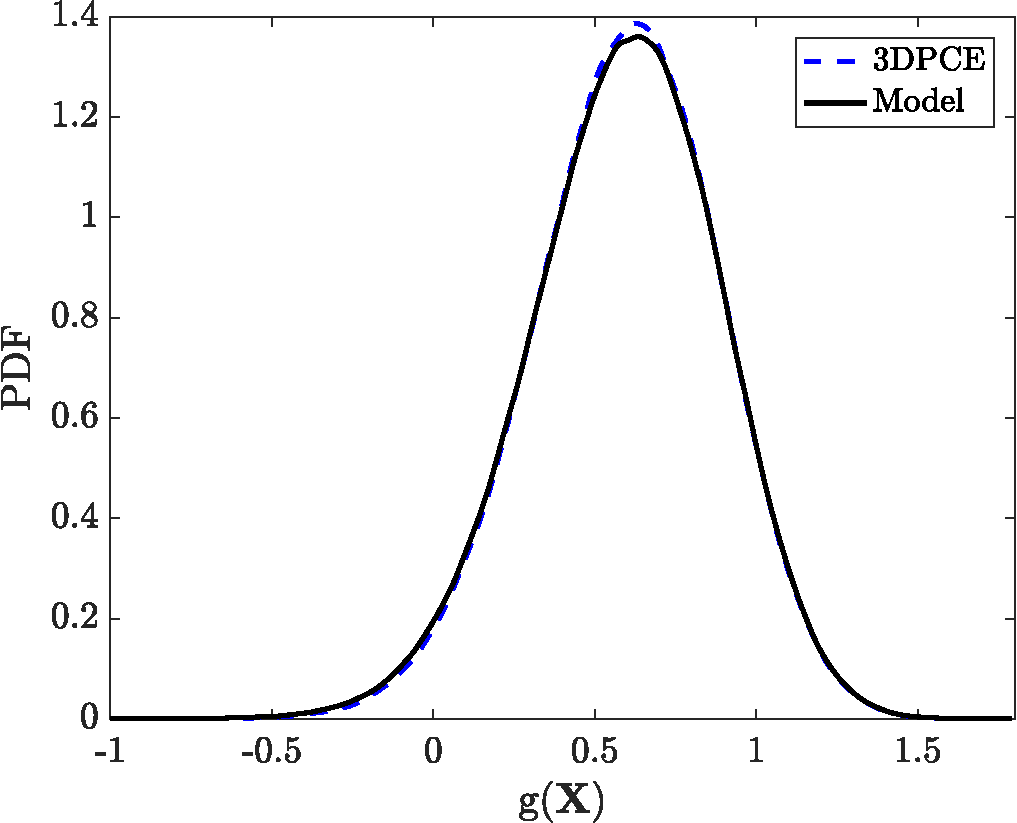
\includegraphics[width=0.48\textwidth]{./Figures/pdf_comp_oscillator}
\caption{Left: Logarithm of $\epsilon_{\mbox{\tiny{LOO}}}$ is plotted against sample size for 
PCEs constructed in 3, 5, and 6 dimensions to compare their convergence characteristics. 
Right: PDF of the limit state function is plotted using the actual function in~\eqref{eq:limit}
and the third-order PCE.}
\label{fig:conv_osc}
\end{center}
\end{figure}

To verify the accuracy of the third-order PCE, we estimate the relative L-2
norm of the difference between predictions of  $g(\bm{X})$, obtained using the
actual function in \eqref{eq:limit} and the 
PCE using \eqref{eq:l2}, and a validation test suite. The test suite comprised
model evaluations at 1000 independent Monte-Carlo samples in the full 
parameter space. The value of $\epsilon_{\mbox{\tiny{L-2}}}$ 
was found to be 0.0835 i.e. the third-order PCE is accurate within 8.36$\%$.
Furthermore, the accuracy is assessed in a probabilistic sense by comparing
in Figure~\ref{fig:conv_osc}~(right),
PDFs of $g(\bm{X})$, obtained using the full-surrogate, reduced-order 
surrogates constructed 3 and 4 dimensions, and a normalized histogram based
on model evaluation in the validation test suite. The three PDFs are observed
to be in excellent agreement with each other as well as the model-based
histogram. Hence, the ROS constructed using the methodology
presented in section~\ref{sec:method} could be used reliably to 
quantify the uncertainty in $g(\bm{X})$ with reduced effort.

\subsection{Semilinear elliptic PDE with random source term}

We consider the following semilinear elliptic PDE: 
\begin{equation}\label{eq:semilinear}
\begin{aligned}
-\kappa \Delta u + c u^3 &= q \quad \text{in } \Omega,\\
 u &= 0 \quad \text{on } \partial \Omega.
\end{aligned}
\end{equation}
Here $\Omega = (0, 1)\times(0,1)$, 
$u$ is the state variable, and $\kappa$ and $c$ are coefficients of the diffusion term
and the nonlinear term in the above equation respectively. 
We consider uncertainties in $\kappa$, $c$, and the source term. 
The right hand side function $q$ is defined by 
\be
q(x, y) = 
\sum\limits_{i=1}^{N=8}\alpha_i\sin\left(\frac{i\pi x}{8}\right)
                               \cos\left(\frac{i\pi y}{8}\right),
\label{eq:source}
\ee
where $\alpha_i$, $i = 1, \ldots, 8$ are random coefficients.
%
Hence, $u~=~u(\vec{\theta})$, where $\vec{\theta} = 
(\kappa,c,\alpha_1,\alpha_2,\ldots,\alpha_{8})^T$ is the vector
of uncertain parameters. Distributions of the uncertain
input parameters are tabulated in Figure~\ref{fig:elliptic}~(left).
The solution of~\eqref{eq:semilinear} for
a fixed set of values of the uncertain parameters is also 
illustrated.

\begin{figure}[htbp]
\begin{center}
\begin{minipage}[htbp]{.25\linewidth}
\vspace{0pt}
%\centering
\hspace{-25mm}
\begin{tabular}{cl}
\toprule
$\theta_i$ & \textbf{Distribution} \\ 
\bottomrule
$\kappa$ & $\mathcal{U}$[0.05,0.1] \\
$c$ & $\mathcal{U}$[1.0,2.0] \\
$\alpha_i$ & $\mathcal{U}$[0.0,4.0] \\
\bottomrule
\end{tabular}
\end{minipage}
\hspace{-20mm}
\begin{minipage}[htbp]{.25\linewidth}
\vspace{0pt}
%\centering
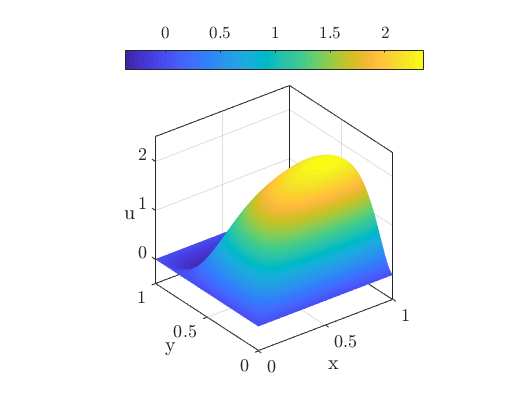
\includegraphics[width=3.0in]{./Figures/u_soln.png}
\end{minipage}%
\end{center} 
\caption{Left: Table providing distributions of the individual
uncertain parameters in~\eqref{eq:semilinear}. Right: Solution
of the 2D semilinear elliptic PDE~\eqref{eq:semilinear} using
$\kappa$~=~0.075, $c$~=~1.5, and $\alpha_i$~=~4.0}
\label{fig:elliptic}
\end{figure}

We aim to construct a reduced-order surrogate for the following QoI:
\be
\mathcal{F}(\kappa, c, \theta) = \frac{1}{|D|} \int_D u(x; \kappa, c, \theta) \, dx, 
\label{eq:qoi}
\ee
%
where $D$ is the region $[2/5, 3/5] \times [2/5, 3/5] \subset \Omega$, 
and $|D|$ denotes the area of $D$. 
While this model is considerably more complex than the previous numerical
examples, it can still be solved efficiently.
The equation was discretized using finite-differences, and Newton's method
was used to solve the resulting nonlinear system on a (100$\times$100) 2D
cartesian grid.
We computed converged estimates of the Sobol
total-effect index $\mathcal{T}(\theta_i)$, reported 
in Figure~\ref{fig:sense_elliptic}~(left) by solving the above non-linear
system at 500 samples in the 10D parameter space. 
%
\begin{figure}[htbp]
 \begin{center}
  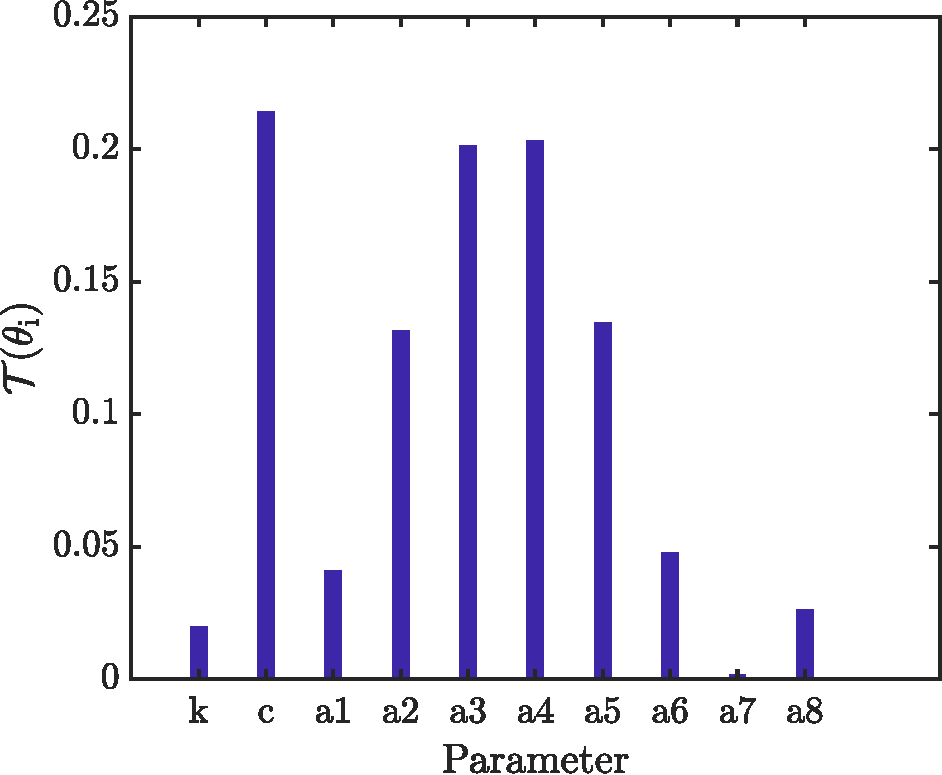
\includegraphics[width=0.46\textwidth]{./Figures/sense_elliptic}
  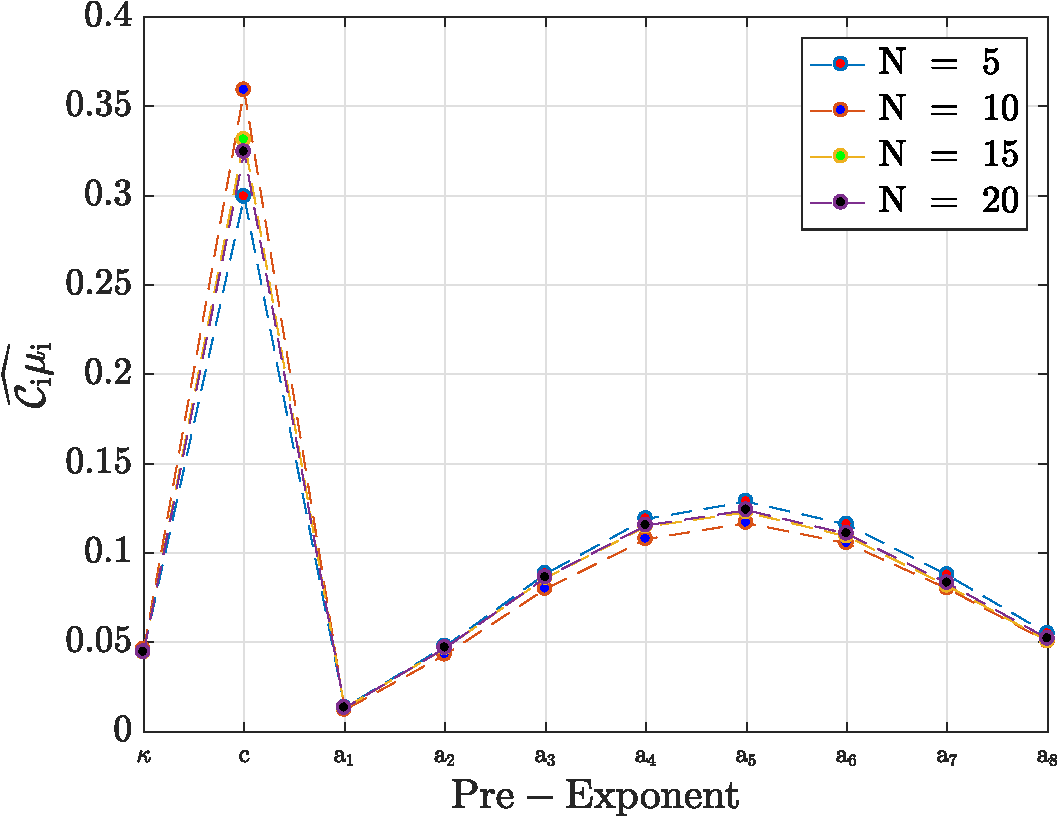
\includegraphics[width=0.48\textwidth]{./Figures/ub_conv_elliptic}
\caption{
Left: Sobol' total sensitivity index, $\mathcal{T}(\theta_i)$ for uncertain parameters in the 
semilinear elliptic PDE~\eqref{eq:semilinear}. Right: 
Estimates of the screening metric ($\widehat{\mathcal{C}_i\mu_i}$) for each uncertain parameter,
obtained using $N$ = 5, 10, 15, and 20 samples in the full parameter space.}
\label{fig:sense_elliptic}
\end{center}
\end{figure}
%
Sensitivity predictions based on the screening metric, $\widehat{\mathcal{C}_i\mu_i}$,
plotted in Figure~\ref{fig:sense_elliptic}~(right), are found to
be in close agreement with $\mathcal{T}(\theta_i)$, even for the case when $N$ = 5. As $N$
is increased from 5 to 20, estimates of the screening metric are observed to converge.
Based on the trends observed in Figure~\ref{fig:sense_elliptic}, it can be said that
the uncertainty in the QoI in \eqref{eq:qoi} is largely dependent on $c$, 
$\alpha_2$, $\alpha_3$, $\alpha_4$, and $\alpha_5$. These observations underscore the
potential for computational gains by constructing an ROS in the 5D parameter space. We 
illustrate the comparison of convergence characteristics of the PCEs constructed in the
full parameter space (10D) and the reduced space (5D) in Figure~\ref{fig:conv_elliptic} (left). 
As expected, the ROS converges considerably faster. Using model evaluations at 90
sample points, $\epsilon_{\mbox{\tiny{LOO}}}$ is found to be two orders of magnitude
smaller than that in the case of full-surrogate ($\mathcal{O}(10^{-4}$) versus
$\mathcal{O}(10^{-2}$)). 
Consequently, the computational effort for constructing the ROS in the present test problem
is expected to be much smaller. 
%
\begin{figure}[htbp]
 \begin{center}
  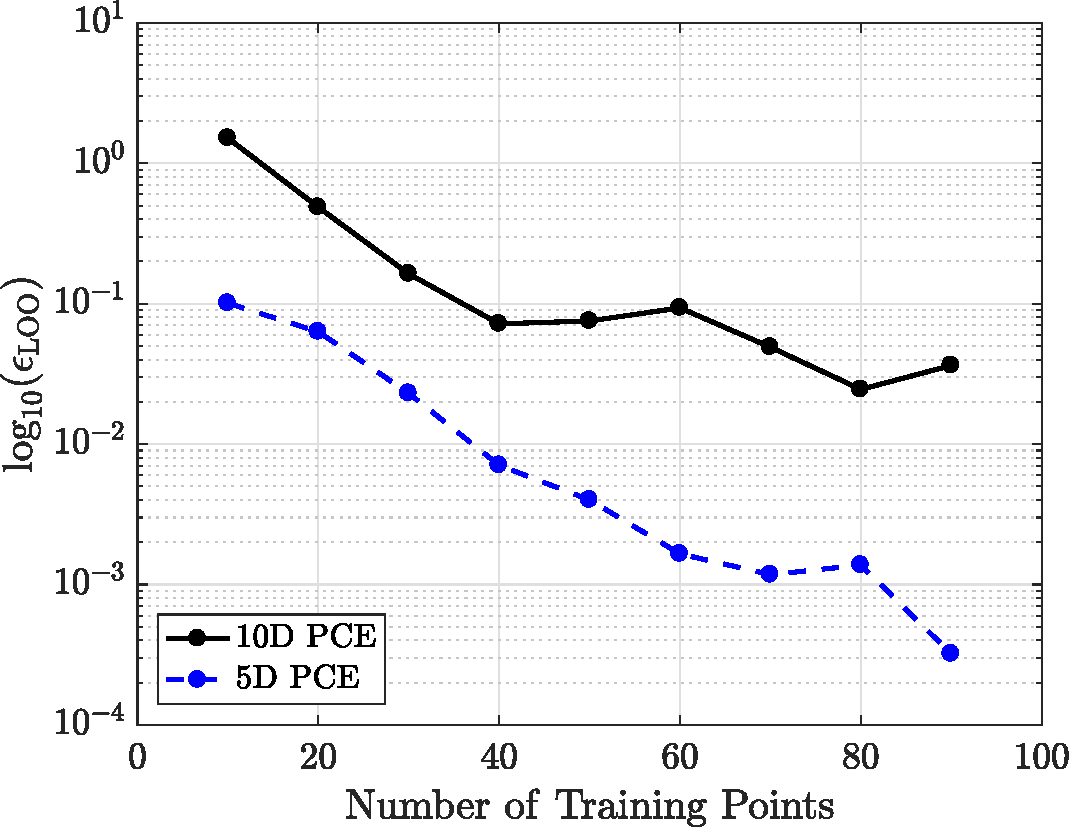
\includegraphics[width=0.48\textwidth]{./Figures/err_samples_elliptic}
  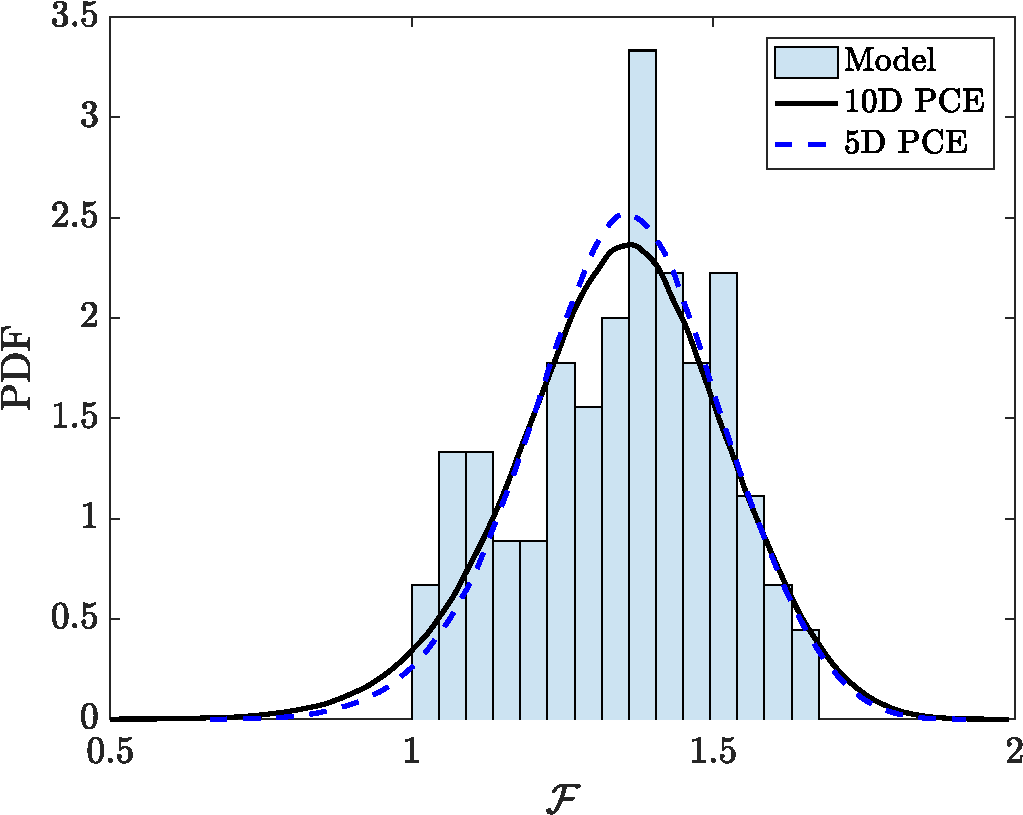
\includegraphics[width=0.48\textwidth]{./Figures/pdf_comp_elliptic}
\caption{Left: Logarithm of $\epsilon_{\mbox{\tiny{LOO}}}$ is plotted against sample size for 
PCEs constructed in 10 and 5 dimensions to compare their convergence characteristics. 
Right: PDF of the QoI, $\mathcal{F}(\kappa, c, \theta)$ in~\eqref{eq:semilinear} is
plotted using the full-surrogate and the reduced-order PC surrogate.}
\label{fig:conv_elliptic}
\end{center}
\end{figure}

Once again, we verify the accuracy of the ROS by estimating $\epsilon_{\mbox{\tiny{L-2}}}$
using model evaluations at 1000 independent Monte-Carlo samples in the 10D parameter
space. The ROS was found to be accurate
within 5$\%$. In order to bolster confidence in the ROS, we compare PDFs of the QoI
as well as a normalized histogram plot based on sparse model evaluations in the  
validation test-suite, in 
Figure~\ref{fig:conv_elliptic}~(right). While the two PDFs are in favorable agreement,
the modal estimate and the spread in the QoI based on the histogram is also captured
by them. Hence, the ROS could be used with a reasonable degree of confidence to
quantify the uncertainty in $\mathcal{F}(\kappa, c, \theta)$ thereby leading to
a computational advantage in this case.































